\begin{figure}[!t]
	\centering
	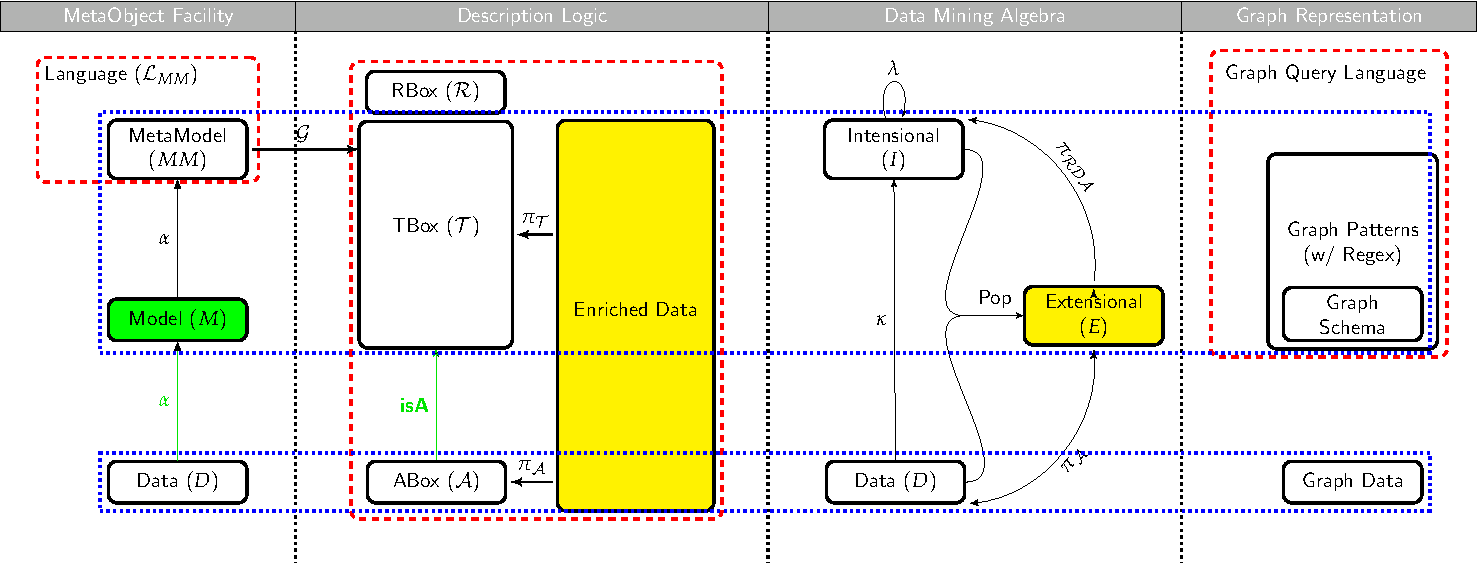
\includegraphics[width=\textwidth]{fig/02models/taonta}
	\caption{A coarse view of all the query languages that have been analysed so far. The rightmost column condenses all the feature  belonging to graph query languages. This picture shows that, while other data models and query languages have a }
	\label{fig:taonta}
\end{figure}
\section{Conclusions}

Structured and semistructured
models point out that a schema can be externally represented, and that (semi)structured data can be represented without the constraints provided by a specific schema, thus allowing a more flexible approach to data integration between different representations. Moreover, the analysis of unstructured data revealed that their translation into a representation of choice depends on a specific scenario, similarly to the adoption of a specific schema to semistructured data.

On the other hand, all the non-graph model fail to represent explicit relations between different data and are all affected by semantic overloading: this last problem will be solved by the property graph model. On the other hand, these data model representations failed to provide a valid representation of nested data structure for data mining and data aggregation purposes. As a consequence, a proper model extending both the semistructured data representation and the graph model is required. The study of the semistructured models allow a generalization of both the object-oriented and relational model in Chapter \vref{cha:graphsdef}: the association between attribute and value for each tag, tuple or object are going to be generalized into a \texttt{MultiMap} instead of a single \texttt{Map}.

Finally, we completed the analysis of several types of query languages: those are roughly subsumed by Figure \ref{fig:taonta}. At the very beginning of this thesis, we were trying to find a valid  representation of semi-structured data, and recognized that the meta-level abstraction  was the ideal place to put such query languages. Still, at this abstraction level it was not clear which query language should have been used. Then, we analysed the Description Logic framework (Definition \vref{def:dlonta}), which is currently used for data integration, and we observed that, even though this language can be used to model and check properties of a given data model, it fails to reproduce data transformation operations. Then, we moved to analyse proper graph query languages: we firstly observed that simple data graphs could be used for the graph data alignment process (Section \vref{sss:gdi}), thus including the more expressive graph traversal and pattern query languages that have been already considered. Then, we introduced graph grammars, thus allowing to introduce the pattern matching and rewriting process that happens in proper graph query languages, allowing to represent most of the possible operations over graph data structures. As showed by Figure \ref{fig:taonta}, as opposed to other query languages and data models where each different abstraction or representation levels requires diverse data operations and representations, graph data structures allow to make all these distinction collapse, thus allowing to reduce the number of the required operations.
